\documentclass[11pt]{article}
\usepackage{amsfonts}
\usepackage{hyperref}
\usepackage{graphicx,subfigure}
\usepackage{epsfig}
\usepackage{hyperref}
\usepackage{amsmath}
\usepackage{amssymb}
\usepackage{algorithm}
\usepackage{algorithmic}
\usepackage{url}
\usepackage{enumerate}
\usepackage{amsfonts}
\usepackage{boxedminipage}
\usepackage{xcolor}
 \usepackage{framed}

\usepackage{tcolorbox}

\usepackage{rotating}
\usepackage{soul}
\usepackage{mathtools}

\usepackage{array}
\usepackage{multirow}
\usepackage{color}
\usepackage{tikz}


\usepackage{mathabx}
\usepackage{tabularx,ragged2e,booktabs,caption}
\usepackage{enumitem}

\usepackage{cancel}
\usepackage{ulem,lipsum}
\usepackage{dsfont}

\newcommand{\overbar}[1]{\mkern 1.5mu\overline{\mkern-1.5mu#1\mkern-1.5mu}\mkern 1.5mu}

\oddsidemargin=0.15in
\evensidemargin=0.15in
\topmargin=-.5in
\textheight=9in
\textwidth=6.25in

\DeclarePairedDelimiter{\floor}{\lfloor}{\rfloor}
\DeclarePairedDelimiter{\ceil}{\lceil}{\rceil}
\DeclareGraphicsExtensions{.gif, .ps, .eps, .png}
\DeclareGraphicsRule{.gif}{png}{}{`convert #1 'png:-'}

\DeclareGraphicsExtensions{.gif, .ps, .eps, .png}
\DeclareGraphicsRule{.gif}{png}{}{`convert #1 'png:-'}

\newcommand{\inprod}[2]{\left\langle #1,#2\right\rangle}
\newcommand{\norm}[1]{\left\| #1\right\|}
\newcommand{\pmat}[1]{\begin{pmatrix} #1\end{pmatrix}}
\newcommand{\cB}{\mathcal{B}}
\newcommand{\bN}{\mathbb{N}\,}

\newcommand*{\vertbar}{\rule[-1ex]{0.5pt}{2.5ex}}
\newcommand*{\horzbar}{\rule[.5ex]{2.5ex}{0.5pt}}

\newcommand{\R}{\ensuremath{\mathbb{R}}}
 % \newcommand{\E}{\ensuremath{\mathbb{E}}}
 \newcommand{\N}{\ensuremath{\mathbb{N}}}
 %newcommand{\C}{\ensuremath{\mathbb{C}}}
 \newcommand{\Tr}{\ensuremath{\top}}
 \newcommand{\Prob}{\ensuremath{\mathbb{P}}}
 \newcommand{\Nc}{\mathcal{N}}
  \newcommand{\Ac}{\mathcal{A}}
  \newcommand{\Dc}{\mathcal{D}}

 % IML
 % ----
 \newcommand{\Xc}{\mathcal{X}}
 \newcommand{\Yc}{\mathcal{Y}}
 \newcommand{\Hc}{\mathcal{H}}
%\newcommand{\inner}[2]{{\left\langle #1\,,\,#2 \right\rangle}}

 % ---

%\newcommand{\norm}[1]{\left|\left| #1 \right|\right|}


\newcommand{\plim}{\stackrel{p}{\rightarrow}}
\newcommand{\aslim}{\stackrel{a.s.}{\rightarrow}}
\newcommand{\dlim}{\stackrel{d}{\rightarrow}}

% distributed as
\newcommand{\iid}{\stackrel{\text{iid}}{\sim}}
\newcommand{\ind}{\stackrel{\text{ind.}}{\sim}}
\newcommand{\indep}{\stackrel{\text{indep.}}{\sim}}
%\newcommand{\V}[1]{\mathbf{#1}}
\newcommand{\Vhat}[1]{\ensuremath{\hat{\mathbf{#1}}}}

\title{{\large{Introduction to Machine Learning (67577) \\
\vphantom{} The PAC Theory of Statistical Learning - Part II}}}

\date{Special Covid-19 edition, 4/2020}

\usepackage{graphicx,subfigure}
% As of 2010, we use the hyperref package to produce hyperlinks in the
% resulting PDF.  If this breaks your system, please commend out the
% following usepackage line and replace \usepackage{icml2011} with
% \usepackage[nohyperref]{icml2011} above.
\usepackage{hyperref}

% \usepackage{icml2011}

\usepackage{amsmath}
\usepackage{amssymb}

\usepackage{algorithm}
\usepackage{algorithmic}
\algsetup{indent=2em}


%% \usepackage{rotating}
%% \usepackage{array}
%% \usepackage{multirow}
%% \usepackage{color}

%% \usepackage{tikz}

\usepackage{url}

\newtheorem{definition}{Definition}
\newtheorem{lemma}{Lemma}
\newtheorem{corollary}{Corollary}
\newtheorem{theorem}{Theorem}
\newtheorem{proposition}{Proposition}
\newtheorem{assumption}{Assumption}
\newtheorem{example}{Example}
\newtheorem{remark}{Remark}
\newtheorem{claim}{Claim}
\newtheorem{exercise}{Exercise}
\newtheorem{discussion}{Discussion}


\newcommand{\gb}[1]{{\boldsymbol{#1}}}
\newcommand{\valpha}{\gb{\alpha}}
\newcommand{\vmu}{\gb{\mu}}
\newcommand{\vnu}{\gb{\nu}}
\newcommand{\vxi}{\gb{\xi}}
\newcommand{\vtheta}{\gb{\theta}}
\newcommand{\vrho}{\gb{\rho}}
\newcommand{\vbeta}{\gb{\beta}}
\newcommand{\vtau}{\gb{\tau}}
\newcommand{\vbalpha}{\gb{\alpha^\star}}
\newcommand{\vbbeta}{\gb{\beta^\star}}
\newcommand{\vtalpha}{\gb{\tilde{\alpha}}}
\newcommand{\vlambda}{\gb{\lambda}}
\newcommand{\slambda}{\bar{\vlambda}}
\newcommand{\stheta}{\bar{\vtheta}}
\newcommand{\vphi}{\gb{\phi}}
\newcommand{\vsigma}{\gb{\sigma}}

\newcommand{\x}{{\mathbf x}}
\newcommand{\y}{{\mathbf y}}
\newcommand{\z}{{\mathbf z}}
\newcommand{\w}{{\mathbf w}}
\newcommand{\bw}{\bar{\w}}
\newcommand{\bF}{\bar{F}}
\renewcommand{\v}{{\mathbf v}}
\renewcommand{\u}{{\mathbf u}}
\newcommand{\e}{{\mathbf e}}
\newcommand{\bsig}{{\mathbf \sigma}}
\newcommand{\rE}{{\mathbf E}}
\newcommand{\sgn}{{\mathrm{sgn}}}
\newcommand{\cF}{{\cal F}}
\newcommand{\pr}{\mathbb{P}}
\newcommand{\rV}{{\mathrm {Var}}}
\newcommand{\tr}{{\mathrm{tr}}}
\newcommand{\trans}{\dagger}
\newcommand{\diag}{{\mathrm{diag}}}
\newcommand{\lspan}{{\mathrm{span}}}
\renewcommand{\r}{{\mathbf{r}}}
\newcommand{\tL}{\tilde{L}}
\newcommand{\hL}{\hat{L}}

\newcommand{\cD}{\mathcal{D}}
\newcommand{\bE}{\mathbb{E}\,}


\newcommand{\BlackBox}{\rule{1.5ex}{1.5ex}}
\newenvironment{proof}{\par\noindent{\bf Proof\ }}{\hfill\BlackBox\\[2mm]}

\newcommand{\reals}{\mathbb{R}}
\newcommand{\Y}{\mathcal{Y}}
\newcommand{\X}{\mathcal{X}}
\renewcommand{\H}{\mathcal{H}}
\newcommand{\E}{\mathbb{E}}
\newcommand{\D}{\mathcal{D}}
\newcommand{\V}{\mathcal{V}}
%\newcommand{\U}{\mathcal{U}}
\newcommand{\F}{\mathcal{F}}
\newcommand{\inner}[1]{\langle #1 \rangle}
\newcommand{\half}{\frac{1}{2}}
\newcommand{\thalf}{\tfrac{1}{2}}
\newcommand{\eqdef}{\stackrel{\mathrm{def}}{=}}
\newcommand{\err}{\mathrm{err}}
\newcommand{\opt}{\mathrm{opt}}
\newcommand{\herr}{\widehat{\err}}
\newcommand{\hopt}{\hat{\opt}}
\newcommand{\eopt}{\epsilon_{\mathrm{opt}}}
\newcommand{\eapp}{\epsilon_{\mathrm{app}}}
\newcommand{\eest}{\epsilon_{\mathrm{est}}}
\newcommand{\halg}{\tilde{h}}
\newcommand{\empf}{\hat{F}_{\lambda}}
\newcommand{\T}{\mathrm{time}}
\newcommand{\erf}{\mathrm{erf}}
\newcommand{\sig}{\mathrm{sig}}
\newcommand{\poly}{\mathrm{poly}}

\newcommand{\rank}{\mathrm{rank}}
\newcommand{\supp}{\mathrm{supp}}
\newcommand{\spn}{\mathrm{span}}
\newcommand{\image}{\mathrm{image}}


\DeclareMathOperator*{\argmin}{argmin} % Declares argmin and ensures super and subscripts are located nicely above/below such as in \min
\DeclareMathOperator*{\argmax}{argmax} % Declares argmin and ensures super and subscripts are located nicely above/below such as in \min
\DeclareMathOperator*{\prob}{\mathbb{P}}

\renewcommand{\eqref}[1]{Equation~(\ref{#1})}
\newcommand{\figref}[1]{Figure~\ref{#1}}
\newcommand{\secref}[1]{Section~\ref{#1}}
\newcommand{\thmref}[1]{Theorem~\ref{#1}}
\newcommand{\lemref}[1]{Lemma~\ref{#1}}
\newcommand{\defref}[1]{Definition~\ref{#1}}
\newcommand{\corref}[1]{Corollary~\ref{#1}}

%\newcommand{\comment}[1]{\textcolor{red}{\textbf{#1}}}
\newcommand{\mathcomment}[1]{\color{red}{\textbf{#1}}}

\newcommand{\indct}[1]{\boldsymbol{1}\!\left[ #1 \right]}

\newcommand{\blambda}{\bar{\lambda}}
\newcommand{\bA}{\bar{A}}
\newcommand{\bI}{\bar{I}}

\newcommand{\vect}{\mathrm{vec}}


\newcommand{\coursename}{Introduction to Machine Learning (67577)}

\newcommand{\handout}[5]{
%   \renewcommand{\thepage}{#1-\arabic{page}}
   \noindent
   \begin{center}
   \framebox{
      \vbox{
    \hbox to 5.78in { {\bf \coursename}
         \hfill #2 }
       \vspace{4mm}
       \hbox to 5.78in { {\Large \hfill #5  \hfill} }
       \vspace{2mm}
       \hbox to 5.78in { {\it #3 \hfill #4} }
      }
   }
   \end{center}
   \vspace*{4mm}
}

\newcommand{\notes}[5]{
%   \renewcommand{\thepage}{#1-\arabic{page}}
   \noindent
   \begin{center}
    \hbox to 5.78in { {\bf \coursename}  \hfill #2}
       \vspace{14mm}
       \hbox to 5.78in { {\Large \hfill #5  \hfill} }
   \end{center}
   \vspace*{4mm}
}

% Lecture notes:
\newcommand{\lecture}[5]{\handout{#1}{#3}{Lecturer:
#4}{Scribe: #5}{Lecture #1: #2}}

\newcommand{\recitation}[5]{\handout{#1}{#3}{#4}{ #5}{Recitation #1: #2}}

% Exam:
\newcommand{\exam}[1]{\handout{#1}{}{}{}{Exam}}
\newcommand{\homeexam}[2]{\handout{#1}{}{}{Due:
#2}{Home Exam}}
\newcommand{\examanswer}[1]{\handout{X}{}{by: #1}{}{Exam - Answers}}

% New exercise
\newcommand{\problemset}[2]{\handout{#1}{}{}{Due:
#2}{Problem Set #1}}

% School solution
\newcommand{\solution}[2]{\handout{#1}{}{}{Written by: #2}{Problem Set #1 - Solution}}

% Submitted solution
\newcommand{\exanswer}[2]{\handout{#1}{}{by: #2}{}{Problem Set #1 - Answers}}

\begin{document}
\maketitle

\tableofcontents
\pagebreak


\part{Recap of previous lecture}

\section*{PAC Theory so far}

Make sure you've read the previous handout (PAC Part I). Recall that we are
developing a theory of ``learning from previous examples'' or ``generalizing
from previous examples'', which suggests a mathematical model for what it
means to learn, what is learnable and what isn't learnable, how to learn when
learning is possible, and what's the minimal number of training samples we need
to learn. All for {\bf supervised batch learning}.

\subsection*{Our framework and The Learning Game}



\paragraph{Framework.}

 Our task is to design a learning algorithm (a "learner"), which we denote by $\mathcal{A}$. For a given sample size $m$, $\mathcal{A}$  is a map from the training sample 
\[S=((x_1,y_1),..,(x_m,y_m)) \in (\X\times \Y)^m\]
where each $\mathbf{x}_i$
to an {\bf hypothesis class}  $\Hc\subset \Y^\X$. We write
$\Ac:(\X\times\Y)^m\to \Hc$ so that $\Ac:S\mapsto h_S\in\Hc$.

We're thinking of classification problems now, so in this lecture $\mathcal{Y}=\{\pm 1\}$, but everything here can be generalized.
The {\bf data generation model} we assume is probabilistic. 
We assume that there is an unknown distribution $\mathcal{D}$ over
$\mathcal{X}$.
 We assume that each sample - both in the training set and in the test set - is sampled
 according to $\mathcal{D}$ independently from any other sample before of after
 it. For the labels $y$, we assume a function $f:\mathcal{X}\to\mathcal{Y}$ such
 that for each sample $x\in\mathcal{X}$, the corresponding label is $y=f(x)$. We
 further assume (the {\bf ``realizability assumption''}) that $f$ is
 $\Dc$-almost-everywhere equal to some $h^*\in\Hc$, namely that $\Dc\left(
   \left\{ x\in\X\,|\, f(x)=h^*(x)  \right\}
 \right)=1$.
In particular, for our training data, we have $y_i = f(x_i)$ for $i=1,\ldots,m$. 
Finally, for a candidate prediction rule $h\in\Hc$ that our learner may produce,
we will measure the generalization performance of $h_S$ - how well it will perform on future unseen samples - by simply using the expected misclassification rate 
$$
L_{\D,f}(h) ~\eqdef~ \prob_{x \sim \D}[h(x) \neq f(x)] \,.
$$
Note that using this notation, the Realizability Assumtion can be written like
this: we assume that the labeling function $f:\X\to\Y $ is such that
$\exists h^*\in\Hc$ with $L_{\D,f}(h^*)=0$.


\paragraph{The Learning Game.} 
The definition of PAC-learnability is more easily understood by thinking about
supervised batch learning as a ``game between us and Nature''. 
Fix desired accuracy $\epsilon>0$ and confidence $\delta>0$. Fix
   an hypothesis class $\Hc \subset \Y^\X$. 
 We play a game against Nature, with random payoff.
  \begin{itemize}
    \item We choose a sample size $m$ and a learner $\Ac:(\X,\Y)^m \to \Hc$. 
    $m$ depends on $(\epsilon,\delta)$.
       \item Nature knows our strategy, and, after us, chooses strategy that consists of a probability distribution $\D$ over $\X$, and a label function {\bf from the specified hypothesis class} $f\in\Hc$. 
     That is, Nature's strategy can depend on $\epsilon,\delta,\Hc$ specified, and also on the $m,\Ac$ we chose. 
    \item A sample $S$ of size $m$ is drawn according to $\D$ and is labeled
      according to $f$
    \item The sample $S$ is fed into $\Ac$ to produce a prediction rule
      $h_S=\Ac(S)$. Note that $h_S\in\Hc$.
    \item The payoff is $L_{\D,f}(h_S)$. It is random since $S$ is random and
      therefore $h_S$ is random.
    \item We are going to assume Nature is ``cruel'' and does her best to win.
      So we'll look for learners $\Ac$ that have a {\bf guaranteed maximal 
      loss} $L_{\D,f}(h)$ {\bf for any} strategy $\D,f$ that Nature might play.
      \item To determine if we were successful in the game, we play the game many many times 
      (both us and Nature play the same strategies, just the training samples drawn are different).
      We count and calculate the probability, over the random draws of training samples $S$, of the event
      $\{ S \sim \D^m \,\big |\,L_{\D,f}(h_S)\leq \epsilon \}$. If this probability is found to be 
      larger than $1-\delta$, that is, if 
      the learner $\Ac$ we chose was Probably Approximately correct with accuracy $\epsilon$ and confidence $\delta$ - against Nature's best strategy - {\bf we say that we've been successful (with regards to the parameters $\epsilon,\delta$) and hypothesis class $\Hc$}.
\end{itemize}

We saw that the definition of PAC learnability of an hypothesis class $\Hc$
(coming next) is equivalent to the following statement: We are able to ``win''
against Nature, for any $\delta,\epsilon>0$, regardless of how Nature plays.


\subsection*{PAC Learnability and Sample Complexity of an hypothesis class $\Hc$}

Slowly and gradually, in the last lecture we unpacked the following
definitions:

\begin{definition}
\begin{enumerate}
\item
A hypothesis class $\Hc$ is {\bf PAC Learnable} if there exists a function $\tilde{m}_\Hc : (0,1)^2 \to \N$ and a learning algorithm $\Ac$ with the following property:
For every $\epsilon,\delta \in (0,1)$ and for every distribution $\D$ over $\X$, and for every labeling function 
$f:\X\to\{\pm 1\}$ that satisfies $L_{\D,f}(h^*)=0$ for some $h^*\in\Hc$, when running the learning algorithm $\Ac$ on $m\ge \tilde{m}_\Hc(\epsilon,\delta)$ i.i.d. examples generated by $\D$ and labeled by $f$, the algorithm returns an hypothesis $h_S=\Ac(S)$ such that, with probability of at least $1-\delta$ (over the choice of the training samples), we have
$
L_{\D, f}(h_S) \le \epsilon
$. 
\item For a PAC learnable hypothesis class, we define the {\bf Sample Complexity} of $\Hc$ for specified $\epsilon,\delta$ as the minimal number of samples $\tilde{m}_\Hc(\epsilon,\delta)$ required for the definition to hold with respect to $\epsilon,\delta$. The Sample Complexity function of $\Hc$ is denoted $m_\Hc(0,1)^2\to\mathbb{N}$.
\end{enumerate}
\end{definition}

We defined a Probably Approximately Correct learner and saw that if an
hypothesis class $\Hc$ is PAC-learnable, this just means that for any $0<\epsilon,
\delta<1$ we are able to
find a Probably Approximately correct learner $\Ac$ with accuracy $\epsilon$ and
confidence $\delta$, regardless of $\D,f$ chosen by Nature. 


\section*{VC Dimension}

{\bf Definition:} Let $C\subset\X$ be a subset of the sample space and let $h:\X\to\Y$ be some hypothesis. 
We define the {\bf restriction} of $h$ to $C$, denoted $h_C:C\to\Y$, by $h_C(x)=h(x)$, for $x\in C$.
\\~\\
{\bf Crucial observation:} As long as $\Hc$ contains {\bf any} set $C$ of size
$2m$ with the property that $\{h_C\,|\,h\in\Hc\} = \Y^C$, then we cannot learn with a training sample of size $m$. It follows that the {\bf maximal size} of such a set $C$ in $\Hc$ is a {\bf critical quantity}: (i) it gives us a lower bound on $m_\Hc$, the minimal sample size needed, and (ii) if the maximal size is $\infty$, namely, if for any $m\in\mathbb{N} \X$ contains such as set $C$ with $|C|>m$, the $\Hc$ is not PAC-learnable!
\\~\\
This is the intuition behind the {\bf lower bound} in the Fundamental Theorem of Statistical
Learning: When trying to learn a function from an hypothesis class $\Hc$, the
{\bf minimal} number of samples needed to learn - using {\bf any} learner (not
just ERM) - is related to the maximal size of a set $C\subset \X$ with the
property that  $\{h_C\,|\,h\in\Hc\} = \Y^C$.

\subsection*{Formal Definition}

Let $C = \{x_1,\ldots,x_{|C|}\} \subset \X$ and let $\Hc_C$ be the restriction of $\Hc$ to $C$, namely,
 $\Hc_C = \{ h_C : h \in \Hc\}$.
 Observe that, always, $|\Hc_C|\leq 2^{|C|}$. The case where the upper bound is
 obtained is the one most interesting to us: 
We will say that $\Hc$ \textbf{shatters} $C$ if $|\Hc_C| =  2^{|C|}$.  
\begin{definition}
The VC dimension of the hypothesis class $Hc$ is defined as 
$$VCdim(\Hc) = \max\{ |C| ~:~ \Hc~\,\,\textrm{shatters}~\,\,C \}\,,$$
that is, the VC dimension is the maximal size of a set $C\subset \X$ such that
$\{h_C\,|\,h\in\Hc\} = \Y^C$.
\end{definition}
We interpret this as the maximal size of a set $C\subset X$ such that 
$\Hc$ gives no prior knowledge on label functions restricted to $C$.
\\
~\\ The {\bf lower bound} part of the Fundamental Theorem of Statistical
Learning gives an explicit connection between $VCdim(\Hc)$ (maximal size of a
subset of $X$ that is shuttered by $\Hc$) and the minimal
number of samples required to produce a PAC learner for $\Hc$ with confidence
$\delta$ and accuracy $\epsilon$ ($ m_\Hc(\epsilon,\delta)$ - the sample
complexity of $\Hc$ at $\epsilon,\delta$): there is a universal constant $C_1$
such that
\[
 C_1
    \frac{d + \log(1/\delta)}{\epsilon} \le m_\Hc(\epsilon,\delta)\]



\subsection*{Examples}
According to the above definition, in order to show that $VCdim(\Hc) = d$ we need to show that:
\begin{enumerate}
\item There exists a set $C$ of size $d$ which is shattered by $\Hc$.
\item Every set $C$ of size $d+1$ is not shattered by $\Hc$.
\end{enumerate}

\subsubsection*{Threshold class}
Consider first $\Hc_{th}$. The set $\{0\}$ is shattered by  $\Hc_{th}$ since $x=0$ can receive both the label 0 and 1, depending on the location of the threshold $\theta$. 

\begin{center}
 
\includegraphics[width=0.5\textwidth,height=0.05\textheight]{ThresholdVC1.png}
\end{center}

In contrast to the above, no two points, $x_1$ and $x_2$ can be shattered because if $x_1 < x_2$ then $y_1 \leq y_2$ and therefore the pair of labels $y_1=1, y_2=0$ is forbidden.

\begin{center}
 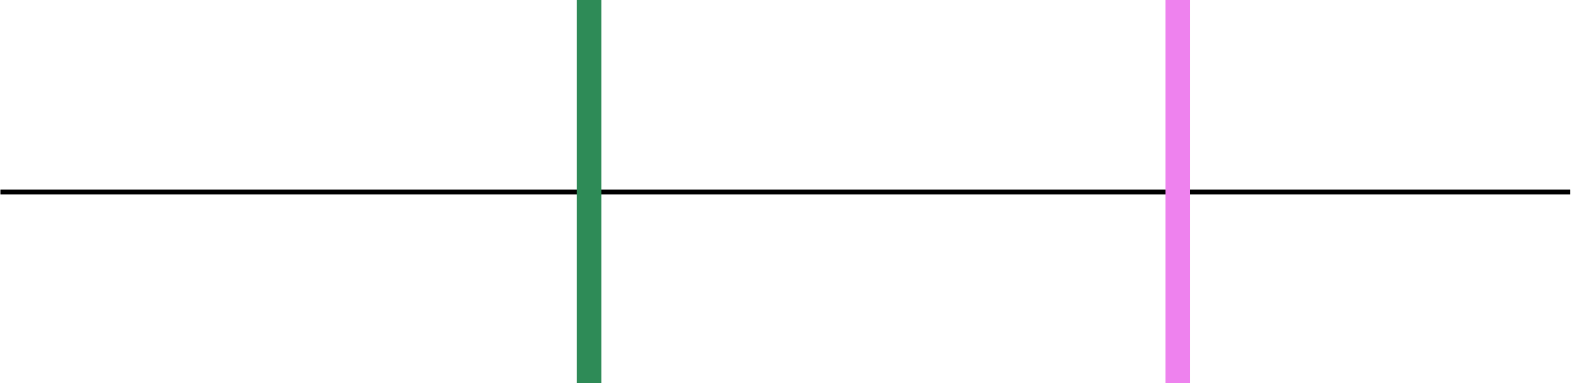
\includegraphics[width=0.5\textwidth,height=0.05\textheight]{ThresholdVC2.png}
\end{center}

\subsubsection*{One-Interval}
Consider the \textbf{One-Interval} hypothesis class over the sample space 
$\X = \reals$. We define $\Hc = \{ h_{a,b} : a < b \in \reals\}$, where $h_{a,b}(x)=1$ if $x \in [a,b]$, and $h_{a,b}(x)=0$ otherwise.
Now, take for example the two points $\{0,1\}$.  We can place the interval over both, over any one of them, or outside $[0, 1]$. Therefore, $\{0,1\}$ is shattered. However, any three points cannot be shattered:
Let $x_1 < x_2 < x_3$, then no single interval can cover $x_1$ and $x_3$ without containing also $x_2$ and therefore the labeling $y_1=1, y_2=0, y_3=1$ is forbidden.

\subsection*{Exercises to help you understand the definition of VC-dimension}

Make sure to solve all these exercises. They will help you understand the
definition of VC-dimension.

\subsubsection*{Axis aligned rectangles}
Consider the \textbf{Axis aligned rectangles} hypothesis class over the sample space 
$\X = \reals^2$. We define $\Hc = \{h_{(a_1,  a_2, b_1 , b_2)}: a_1 < a_2 ~\text{and}~  b_1 < b_2 \}$, 
where $ h_{(a_1, a_2, b_1 , b_2)}(x_1,x_2) = 1$ if $x_1 \in [a_1,a_2]$, and $x_2 \in [b_1,b_2]$, and  $ h_{(a_1, a_2, b_1 , b_2)}(x_1,x_2) = 0$ otherwise. (Convince yourself that a function in this hypothesis class is an indicator of a finite open rectangle aligned with the canonical basis of $\reals^2$.)

\vspace{9mm}

Verify that:
\begin{center}
\begin{tabular}{lr}
Shattered & Not Shattered \\
\begin{tikzpicture}[scale=1]
\fill[blue] (0,1) circle (0.1);
\fill[blue] (1,0) circle (0.1);
\fill[blue] (0,-1) circle (0.1);
\fill[blue] (-1,0) circle (0.1);
\end{tikzpicture} & \hspace{2cm}
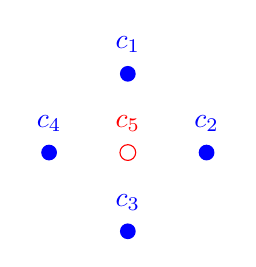
\begin{tikzpicture}[scale=1]
\fill[blue] (0,1) circle (0.1) node[above=4pt] {$c_1$};
\fill[blue] (1,0) circle (0.1) node[above=4pt] {$c_2$};
\fill[blue] (0,-1) circle (0.1) node[above=4pt] {$c_3$};
\fill[blue] (-1,0) circle (0.1) node[above=4pt] {$c_4$};
\draw[red] (0,0) circle (0.1) node[above=4pt] {$c_5$};
\end{tikzpicture}
\end{tabular}
\end{center}
~\\
{\bf Exercise:} show that no set of 5 points can be shattered by the Axis aligned rectangles class. Hint: note that the 3 points $(x_k,y_k)$, $(x_i,y_i)$, and $(x_{k'},y_{k'})$ can not be shattered if $x_k\leq x_i\leq x_{k'}$ and $y_k\leq y_i\leq y_{k'}$.


\subsubsection*{Finite classes}
~\\{\bf Exercise:}
\begin{itemize}
\item Show that the VC dimension of a finite $\Hc$ is at most
$\log_2(|\Hc|)$.
\item  Assume $\Hc$ is finite. Show that there can be arbitrary gap between $VCdim(\Hc)$ and
  $\log_2(|\Hc|)$, namely, construct a finite hypothesis class $\Hc$ over some sample space $\X$ with $VCdim(\Hc) = \log_2(|\Hc|)$ 
  and another finite hypothesis class with $VCdim(\Hc)=1$.  
\end{itemize}

\subsubsection*{Half-spaces through the origin}
Consider the sample space $\X = \reals^d$ and the hypothesis class of half-spaces through the origin
$\Hc = \{ \x \mapsto sign(\inner{\w,\x}): \w \in \reals^d\}$. 

~\\{\bf Exercise:}
\begin{itemize}
\item Show that $\{\e_1,\ldots,\e_d\}$ is shattered
\item Show that any $d+1$ points cannot be shattered (hint: consider the standard basis vectors...)
\item What is $VCdim(\Hc)$?
\end{itemize}

%\subsubsection{Classification trees}
%What is the VC-dimension of a full balanced classification tree with $b$
%levels?





\part{Today's lecture}

\section{Finite Hypothesis Classes are PAC learnable}

We talked about finite hypothesis classes in the previous lecture, and stated a
theorem whereby finite hypothesis classes are PAC learnable, but did not
prove it. Let's recall the details and prove the theorem.

We recall that a finite hypothesis classes can be huge: for example, take $\Hc$ is all the functions from $\X$ to $\Y$ that can be implemented using a Python program of length at most $b$, for $b$ fixed and large. Or, take $\Hc$ to be all the functions from $\X$ to $\Y$ where  $|\X|$ and $|\Y|$ are finite.

\subsubsection{Empirical Risk Minimization}

It turns out that {\bf there is a simple learner that is always successful on finite hypothesis classes} (and on many other hypothesis classes as we will see later).

The idea behind this amazing learning is very simple and natural: try to be as correct as possible on the training data!

Formally, given  a training set $S = (x_1,y_1),\ldots,(x_m,y_m)$ we define the {\bf empirical risk} of a candidate prediction rule $h\in\Hc$ by
$$L_S(h) = \frac{1}{m} |\{i : h(x_i)  \neq y_i\}|\,.$$

Our amazing learning algorithm is simple: on a training sample $S$, it returns $h \in \Hc$ that {\bf minimizes the empirical risk $L_S(h)$.} In other words,
\[
\Ac_{ERM} : S \mapsto \text{argmin}_{h\in\Hc} L_S(h) = \frac{1}{m} \,.
\]
The minimum may not be unique, in which case the algorithm returns one of the minimizers. Our amazing learner is therefore called \textbf{Empirical Risk Minimization (ERM)} learner. We give this important learner its own special notation and denote it by $ERM_\Hc$ instead of $Ac_{ERM}$.

But wait, how do we know that there is a minimum?  Note that $L_S(h)\geq 0$, and we are minimizing over a finite class, so there is a minimum. In fact, under the assumption that Nature plays $f\in\Hc$, we know that for any training sample $S$,  $L_S(f) = 0$ for the particular labeling function that Nature chose. So that the lower bound $0$ is achievable. In other words, under our assumption that $f\in\Hc$, the ERM learner will always return a rule  $h$ with $y_i = h(x_i)$ for $i=1,\ldots,m$. 
Such a rule is called \textbf{Consistent} - it is consistent with the training sample. 


\subsubsection{Learning Finite Classes}

Our main observation concerning finite classes is simple: a {\bf finite} hypothesis
class $\Hc\subset\Y^\X$ is PAC-learnable, using the ERM rule,
with sample complexity at most 
$\log(|\Hc|/\delta)/\epsilon$.

\begin{theorem}
  Fix $0< \epsilon,\delta <1$. If \[m \ge \frac{\log(|\Hc|/\delta)}{\epsilon}\] 
  then for every $\D$ over $\X$ and every $f$ such that $\exists h^*\in\Hc$ with
  $L_{D,f}(H^*)=0$, with probability of at least $1-\delta$ (over the choice of $S$ of size $m$), $L_{\D,f}(ERM_\Hc(S)) \le \epsilon$.
\end{theorem}

In words, the theorem states that a finite hypothesis class $\Hc$ is PAC
learnable with sample complexity $m_\Hc(\epsilon,\delta)\leq
\frac{\log(|\Hc|/\delta)}{\epsilon}$.
The figures below explain schematically the relation between the accuracy, confidence and the sample size for finite classes, as implied by the above theorem.

% \begin{figure}[h!]
% \centering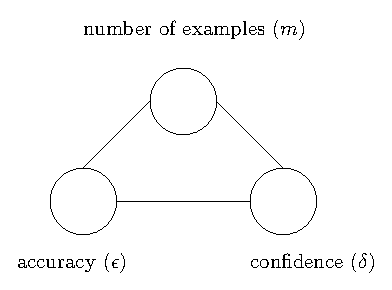
\includegraphics[scale=0.8]{connection_m_eps_delta.eps}
% \end{figure}


  \begin{figure}[h!]
 \centering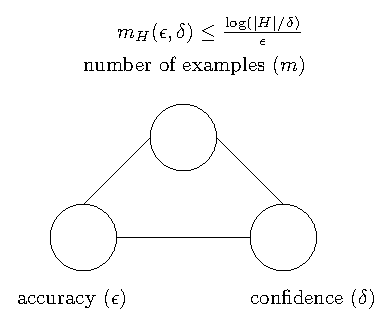
\includegraphics[scale=0.8]{connection_m_eps_delta_finite4.eps}
  \end{figure}


  \begin{figure}[h!]
 \centering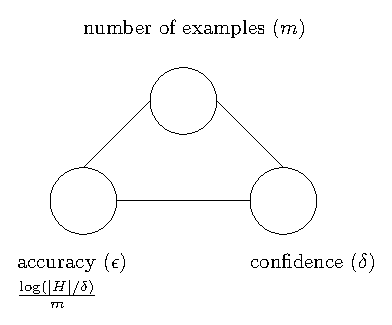
\includegraphics[scale=0.8]{connection_m_eps_delta_finite2.eps}
 \end{figure}


  \begin{figure}[h!]
 \centering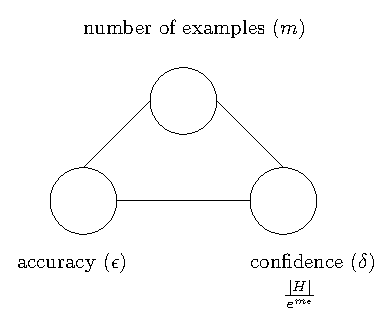
\includegraphics[scale=0.8]{connection_m_eps_delta_finite3.eps}
 \end{figure}

Let us prove the theorem in full (more details can be found in \textit{Understanding Machine Learning} Ch. 2.3.1). For each $S$ our algorithm chooses a hypothesis $ERM_{\Hc}(S)$
Let $\Hc_B$ be the set of "bad" hypotheses,
 \[ \Hc_B = \{h \in \Hc : L_{\D,f}(h) > \epsilon\} \]
and let $S|_x = (x_1,\ldots,x_m)$ be the instances of the training set. We would like to prove:
\[
\D^m(\{ S|_x : ERM_{\Hc}(S)\in \Hc_B \})  \le \delta
\]

Let us denote by $M$ the set of "misleading" samples,
\[M = \{S|_x : \exists h \in \Hc_B, L_S(h)=0\} \]
%
that is, for every input sample $S$ in $M$ there exists an $h$ that in spite of being perfectly correct on that sample, and therefore \textit{could be} chosen by the ERM algorithm as a possible output for that input, its global error is larger than $\epsilon$. In particular, all the $S$'s in the set $\{ S|_x : ERM_{\Hc}(S)\in \Hc_B \}$ belong to $M$ because these are the samples for which our \textit{specific} algorithm chooses a "bad" $h$ (that is, one with $L_{\D,f}(h) > \epsilon$, which means it is in $\Hc$) and being an ERM algorithm, the $h$ it outputs must satisfy $L_S(h)=0$. Therefore:
%
\[\{S|_x : L_{\D,f}(ERM_\Hc(S)) > \epsilon\} \subseteq M \,.\]
We can rearrange the samples in  $M$ according to the $h$'s they share by writing $M$ as:
\[ M = \bigcup_{h \in \Hc_B} \{ S|_x : L_S(h) = 0 \}\]
In this representation, samples in $M$ which share several $h$'s will be counted more than once but since $M$ is a set, this has no effect.
Combining the last two relations we have
\[\{S|_x : L_{\D,f}(ERM_\Hc(S)) > \epsilon\} \subseteq M \]
and using the \textbf{Union Bound}, that is, the fact that for any two sets $A,B$ and a distribution $\D$ we have $\D(A \cup B) \le \D(A) + \D(B) ~$, we get
$$\D^m(\{ S|_x : L_{\D,f}(ERM_\Hc(S)) > \epsilon \}) \le \sum_{h \in \Hc_B} \D^m( \{ S|_x : L_S(h) = 0 \} )\,.$$
Given an $h$, $ \D^m( \{ S|_x : L_S(h) = 0 \}$ is the probability to pull a sample over which $h$ is perfectly correct (has the right labels for all $x_i$'s). 
Since the  $x_i$'s are drawn independently, this probability equals the probability that $h$ will be correct for each of the $x_i$'s separately. 
But the probability that $h$ will be \textit{incorrect} for a random $x$ is exactly $L_{\D,f}(h)$. So the probability that $h$ will be correct for $m$ such $x$'s is $(1-L_{\D,f}(h))^m$. 
We therefore have, for any $h$,
\[ \D^m( \{ S|_x : L_S(h) = 0 \} ) = (1-L_{\D,f}(h))^m \quad \forall h \,.\]
In particular, if $h \in \Hc_B$ then $L_{\D,f}(h) > \epsilon$ and therefore
\[ \D^m( \{ S|_x : L_S(h) = 0 \} ) < (1-\epsilon)^m \quad \forall h \in \Hc_B \,.\]
Substituting this bound above we obtain
\[ \D^m(\{ S|_x : L_{\D,f}(ERM_\Hc(S)) > \epsilon \}) \le \sum_{h \in \Hc_B} (1-\epsilon)^m < |\Hc_B|\,(1-\epsilon)^m  \le  |\Hc|\,(1-\epsilon)^m \,.\]

Finally, using $1-\epsilon \le e^{-\epsilon}$ we conclude:
\[ \D^m(\{ S|_x : L_{\D,f}(ERM_\Hc(S)) > \epsilon \}) ~<~ |\Hc|\,e^{-\epsilon\,m} \,.\]

The right-hand side would be $\le \delta$ if $m \ge
\frac{\log(|\Hc|/\delta)}{\epsilon}$ and therefore we are done. $\blacksquare$

\vspace{5mm}

The figure below illustrates the use of the union bound. Each point is a possible sample $S|_x$. Each colored oval
  represents misleading samples for some $h \in \Hc_B$. The probability
  mass of each such oval is at most $(1-\epsilon)^{m}$. But, the algorithm
  might err if it samples $S|_x$ from any of these ovals.

\begin{center}
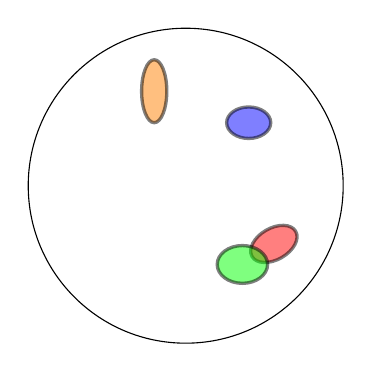
\begin{tikzpicture}[scale=0.4]
\draw (0,0) circle (5);
\filldraw[very thick,color=black,fill=blue,opacity=.5] (2,2) ellipse (0.7 and 0.5);
\filldraw[very thick,color=black,fill=orange,opacity=.5] (-1,3) ellipse (0.4 and 1);
\filldraw[very thick,color=black,fill=red,rotate=30,opacity=.5] (1.5,-3) ellipse (0.8 and 0.5);
\filldraw[very thick,color=black,fill=green,opacity=.5] (1.8,-2.5) ellipse (0.8 and 0.6);
\end{tikzpicture}
\end{center}

\vspace{5mm}

To summarize this section, we have shown the following:
{\bf A finite hypothesis class $\Hc$ is PAC learnable using the ERM learning algorithm, and has a sample complexity  $m_\Hc(\epsilon,\delta)\leq \log(|\Hc|/\delta)/\epsilon$ samples.}

%So, given $\epsilon,\delta \in (0,1)$, all that the learning algorithm needs is to be consistent with the sample (to be an ERM) while the sample size $m$ should satisfy $m\ge m_\Hc(\epsilon,\delta)= \frac{\log(|\Hc|/\delta)}{\epsilon}$.



\section{The Fundamental Theorem of Statistical Learning}

We worked hard to understand the two fundamental definitions above: PAC-Learnability (and sample complexity) of an hypothesis class, and VC-dimension of an hypothesis class. 
\\~\\
Along the way, we saw some connections between these two definitions:
\begin{itemize}
    \item We saw that a finite hypothesis class is PAC-learnable (using the ERM learner)
    with sample complexity \[m_\Hc(\epsilon,\delta)\leq \frac{\log(|\Hc|) + \log(1/\delta)}{\epsilon} \]
    and also that in this case $VCdim(\Hc)\leq \log(|\Hc|)$. Somehow it seems that $VCdim(\Hc)$ is related to an upper bound on $\Hc$ for finite hypothesis classes.
    \item We saw, using a loose argument (the "proof" of No Free Lunch), that $VCdim(\Hc)$ also gives a {\bf lower bound} on the sample complexity $m_\Hc$ of an hypothesis class $\Hc$, and that if $VCdim(\Hc)$ is infinite, that class is not PAC-Learnable. 
\end{itemize}

The surprising, shocking, wonderful truth is that VC-dimension gives a complete and full characterization of PAC-learnabilty and sample complexity of an hypothesis class, and gives a decisive answer to all the questions we posed at various stages along the way (such as which classes are PAC-learnable, with what sample complexity, and with what algorithm, and is there an algorithm that uses the minimal possible sample size.)

The Fundamental Theorem of Statistical Learning states as follows:
\begin{itemize}

\item The PAC-lernability of an hypothesis class is characterized by the \textbf{VC dimension}, a combinatorial property of the class that denotes the maximal size of a sample that can be shuttered by the class.  The characterization is as follows: an hypothesis class is PAC-learnable {\bf if and only if} its VC-dimension is finite.
\item When $VCdim(\Hc)$ is finite (so that $\Hc$ is PAC-learnable and we can ask about its sample complexity), its sample complexity is basically 
\[
m_H(\epsilon,\delta) \sim \frac{VCdim(\Hc)+\log(1/\delta)}{\epsilon}
\]
up to come constants. 
\item The ERM learning rule is a generic (near) optimal learner, in the sense that when a hypothesis class is PAC-learnable, ERM using 
\[
m(\epsilon,\delta) \sim  \frac{VCdim(\Hc)\log(1/\epsilon)+\log(1/\delta)}{\epsilon}
\]
is a Probably Approximately correct learner with accuracy $\epsilon$ and confidence $\delta$.
\end{itemize}

The formal statement of the theorem is as follows: (see   Understanding Machine Learning book, ch. 6.6)
	

  \begin{theorem}[The Fundamental Theorem of Statistical
    Learning] 
    Let $\Hc$ be a hypothesis class of
    binary classifiers with VC-dimension $d\leq \infty$. 
    Then, $\Hc$ is PAC-learnable if and only if $d<\infty$. In this case: (1) there
    there are absolute constants $C_1,C_2$
    such that the sample complexity of $\Hc$ satisfies \[ C_1
    \frac{d + \log(1/\delta)}{\epsilon} \le m_\Hc(\epsilon,\delta) \le
    C_2 \frac{d \log(1/\epsilon) + \log(1/\delta)}{\epsilon} \]
(2) Furthermore, the upper bound on sample complexity is achieved by the ERM learner.
  \end{theorem}

  We already saw the intuition behind the lower bound - how the VC-dimension
  $VCdim(\Hc)$ is related to the {\bf minimal} number of training samples needed
  to PAC-learn the hypothesis class $\Hc$ - using {\bf any} learning algorithm.
\\~\\
To understand the upper bound, we need to understand 
how is it that the ERM learner is a {\bf generic
learning algorithm} that is able to PAC-learn $\Hc$ with a training sample size
again related to the VC-dimension $VCdim(\Hc)$.
\\~\\
Before we discuss the upper bound, let us extend our theoretic framework and
make it much more flexible and realistic.



  \section{Agnostic PAC: Extending our theoretical framework}

  The theoretical framework we developed is not so satisfying, and is
  not such a great theoretical model for ``real'' learning problems, for a few
  reasons:
  \begin{itemize}
    \item {\bf It doesn't model noisy labels.} We have no model for measurement errors. In practice, sometimes even
      though the label for some $\x\in\X$ ``should'' have been $1$ (say), it can
      be measured as $-1$ due to measurement mistake, noise, etc. We want our
      framework to allow for the fact that we may, with low probability, observe the point $x\in\X$
      twice, and get two different labels - namely, observe $(x,+1)$ and later
	sample again and observe $(x,-1)$ - due to noise. 
      \item {\bf The realizability assumption is  unrealistic.} We define
        the hypothesis class.  It is unrealistic to restrict Nature to choose
	from the hypothesis class that we defined. Nature will do as she likes.
      \item {\bf Limited to misclassification loss.} In our framework, we could
	only
	measure the classifier performance using the misclassification loss
	(otherwise known as the $0-1$ loss). We would like to be able to measure
	performance using any loss function we like.
  \end{itemize}

  We now introduce an improved theoretical framework, sometimes know as {\bf
  Agnostic PAC}. It improves on the PAC learning framework and  solves the
  problems above: (i) it allows 
  measurement noise,  (ii) it removes the realizability assumption, and (iii) it
  allow us to specify any loss function. The good
  thing is, as we mention below, the fundamental theorem of statistical learning
  holds in the Agnostic PAC framework as well.


  \subsection{Moving from a probability distribution over $\X$ to a joint
  probability distribution over $\X\times\Y$}

%    \label{D:def} [UML Section 3.2.1]
  Our first step will be to change the probability distribution $\Dc$. For far,
  $\Dc$ was a probability distribution over the sample space $\X$, and the
  labels were determined - deterministically - using the labeling function $f$.
  In our upgraded framework, $\Dc$ will be a probability distribution over
  $\X\times \Y$. This means that when we draw a new random example $(x,y)$ - whether for
  the training sample $S$ or as a test sample - there is randomness in {\bf
  both} $x$ and $y$, and, crucially, it's a {\bf joint} randomness. 
  \\~\\
  We can factor $\Dc$ in two ways, conditioning on $x$ or on $y$. Both are useful for our understanding.
  Let $(X,Y)$ be a random variable taking valued in $\X\times \Y$ whose
  distribution is $\Dc$. 
\begin{itemize}
  \item $\prob(X=x,Y=y)=\prob(X=x)\prob(Y=y|X=x)$. From this perspective, this is a direct
    generalization of our previous framework, where $x$ was random and $y=f(x)$.
    Indeed, we draw $x$ from the marginal distribution with probability
    $\prob(X=x)$ - as we did in the previous framework. We then choose a corresponding 
    label according to the conditional probability $\prob(Y=y|X=x)$. Since the
    marginal random variable $Y$ is a Bernoulli random variable, this means
    there's a function $p:\X\to[0,1]$ such that $\prob(Y=+1|X=x)=p(x)$, namely,
    choosing the label for $x$ is a coin flip with probability $p(x)$. If
    $p(x)=0$ or $p(x)=1$ for some $x$, the label is deterministic and we are
    back to the ``label function'' $f$. But for other values of $p(x)$, whereas
    before the label depended deterministically on $x$, now it is random.
    This models {\bf measurement noise} - the fact that there may be noise in
    the labels, and that the distribution of the noise may change from $x$ to $x$. 
    (This is the perspective of the Logistic Regression classifier you saw in
    the classification lecture, for example. There, we didn't pay attention a
  distribution on $x$ - just assumed the samples are given - and tried to
estimate the conditional probability $\prob(Y=+1|X=x)=p(x)$.)
  \item $\prob(X=x,Y=y)=\prob(Y=y)\prob(X=x|Y=y)$. For this perspective, we
    first draw the label according to a ``coin flip'' -  a Bernoulli random
    variable. Then, each class has its own distribution for the samples $x$. We
    draw the label $x$ from $\prob(X=x|Y=+1)$ or from $\prob(X=x|Y=-1)$, according
    to the label $y$ chosen. (This is the perspective of the LDA classifier you
    saw in homework, for example.) 
\end{itemize}
  
  
\paragraph{Exercise.} Let $\tilde{\D}$ be a distribution on $X$ alone, and let
$f:\X\to\Y$ be a labeling function. Construct an equivalent joint distribution
$\D$ on $\X\times\Y$ such that the random variable $(X,f(X))$, where
$X\sim\tilde{\D}$, has the same distribution over $\X\times\Y$ as $(X,Y)\sim\D$. 
%
\\~\\
How shall we define the loss, when $\Dc$ is a distribution over $\X\times \Y$?
It's simple. Staying (for now) with the misclassification loss, we just define,
for a hypothesis $h:\Xc\to\Yc$,
    \begin{eqnarray} \label{L:def}
        L_\Dc(h) := \Prob_{(x,y)\sim\Dc}\left\{ h(x)\neq y \right\}
        \equiv \Dc\left\{ (x,y)\,|\, h(x)\neq y \right\}
    \end{eqnarray}
    ~\\
    Notice we no longer have a ``ground truth'' labeling function $f$. The
    closest thing we have to $f$  is the conditional probability
    $\prob(Y=y|X=x)$.




\subsection{Removing the realizability assumption}

Recall that in the deterministic labeling case, under the realizability
assumption, we could reach zero generalization error:
\[
    \min_{h\in\Hc} L_{\Dc,f}(h) = L_{\Dc,f}(f)=0\,.
\]
However, in the random labeling case, there is no ``ground truth'' labeling function $f:\Xc\to\Yc$, so
that the realizability assumption no longer makes sense. Due to the measurement
noise, we may no longer be able to reach $0$ generalization loss. This means we
have to change the definition of {\bf accuracy}: we expect the learning
algorithm to output a rule which has generalization loss {\bf at most $\epsilon$
larger than the
minimal possible loss} $\min_{h\in\Hc} L_\Dc(h)$. 
But wait, does a minimum exist? What can we say about this minimum?

%[Bayes optimal predictor - UML section 3.2.1]

\paragraph{Definition: Bayes optimal predictor}
In the recitation you saw the following definition.
    For a given distribution $\Dc$ on $\Xc\times \Yc$ define the {\em Bayes
    optimal predictor} for $\Dc$ by 
    \[
        f_\Dc(x) = 
        \begin{cases}
            1 & \Prob(y=1|x)\geq 1/2\\
            0 & otherwise
        \end{cases}
    \]
~\\
Note that $f_\Dc:\X\to\Y$ is a rule (an hypothesis). However it depends on
$\Dc$, which, according to the rules of the game, we don't know. So $f_\Dc$ is
what is known as an {\bf Oracle Quantity} - if we had an oracle telling us
$\Dc$, then we could classify with $f_\Dc$. Oracle quantities, like this one,
are used to compare the loss of any other rule to the loss of the {\bf best
possible} rule. 
\\~\\
In homework you solved the following
{\bf Exercise.} The Bayes optimal predictor has the best possible generalization
error: 
$ \forall g:\Xc\to\Yc  \,\,,\,\, L_\Dc(f_\Dc)\leq L_\Dc(g) $. 
\\~\\
It follows that for any hypothesis class $\Hc\subset \Y^\X$,
\[
  L_\Dc(f_\Dc) = \min_{h\in \Y^\X} L_\Dc(h)  \leq \min_{h\in\Hc} L_\Dc(h)
\]
and so  $\{L_\Dc(h)\,|\, h\in\Hc\}$ is bounded from below and, glossing over the
difference between minimum and infimum, we can write $\min_{h\in\Hc} L_\Dc(h)$.
~\\
\paragraph{Definition:}
Let $\epsilon>0$.
We say that a rule $h\in\Hc$ is Approximately correct with accuracy $\epsilon$
with respect to the distribution $\Dc$ on $\X\times \Y$ if 
\[
   L_\Dc(h) \leq  \min_{h'\in\Hc} L_\Dc(h') + \epsilon\,,
\]
namely, if $L_\Dc(h)$  is at most $\epsilon$ away from the best possible loss
achievable by {\bf any} hypothesis in $\Hc$. We note again that, in our previous
framework, under the
realizability assumption, the minimal loss is simply $0$ since we {\bf assumed}
the existence of some $h'\in\Hc$ with $L_\Dc(h')=0$.
\\~\\
So, we got rid of the realizability assumption: we no longer assume that Nature
plays a labeling function in the chosen hypothesis class $\Hc$. In fact, we no
longer have a labeling function at all! Nature's strategy just consists of the joint
distribution $\D$ over $\X\times \Y$.

\subsection{Introducing a general loss function}

So we achieved two of the three improvements we wanted: we allow measurement
noise in the labels, and we got rid of the realizability assumption. 
Our last improvement is to allow a general loss function.
% [UML section 3.2.2]
 \paragraph{Definition:  general loss function.}
 A {\bf loss function} is a function $\ell:\Hc \times Z\to[0,\infty)$, where 
 $Z = \X\times\Y$.
For  $z=(x,y)$, we simplify the notation and, instead of the cumbersome notation
$\ell(h,z)$, we simply write  $\ell(h(x),y)$.
\\~\\
We already know well the most common example for classification loss - the
misclassification loss, also known as the  {\bf 0-1 loss}.
\[
    \ell_{0,1}(h,(x,y)):=
    \begin{cases}
        1 & h(x)\neq y\\
        0 & h(x)= y
\end{cases}\,.
\]
\\~\\
Indeed the loss we work with $L_\Dc(h)$ from \eqref{L:def} above can we written
as 
\[
    L_\Dc(h) \equiv \E_\Dc [\ell_{0-1}(h,(x,y))]
\]
where here and below $\E_\Dc[\cdot]$ denotes the expected value according to
$(x,y)\sim \Dc$. 

From here on we will assume a general loss function $\ell$, but will often
have in mind $\ell_{0,1}$.

\paragraph{Definition: generalization loss induced by a general loss function.}
 For a distribution $\Dc$ on $\X\times\Y$ and a loss $\ell:\Hc\times Z\to[0,\infty)$
 (where again $Z=\X\times \Y$) we
 extend Definition \ref{D:def} and define the loss of a rule (hypothesis)
 $h:\X\to\Y$ with respect to $\D$ and $\ell$ as
 \begin{eqnarray*}
     L_\Dc(h) := \E_{z\sim\Dc}[\ell(h,z)]
 \end{eqnarray*}
 where $Z=\Xc\times\Yc$ and $z=(x,y)\in Z$.
\\~\\
How shall we define {\bf accuracy} with respect to a general loss induced by a
general loss function? The definition above (for $0-1$ loss) generalizes
naturally and easily:
%
\paragraph{Definition:}
Let $\epsilon>0$.
We say that a rule $h\in\Hc$ is Approximately correct with accuracy $\epsilon$
with respect to the distribution $\Dc$ on $\X\times \Y$, the loss function
$\ell:\Hc\times (\X \times\Y)\to[0,\infty)$ and the hypothesis class $\Hc$ 
if 
\[
  L_\Dc(h) \leq \min_{h'\in\Hc} L_\Dc(h') + \epsilon\,.
\]
Note that now accuracy must be defined with respect to an hypothesis class
$\Hc$.



 \section{Agnostic-PAC learnability}
 Our new framework is called Agnostic-PAC.
 We are now ready to define Agnostic-PAC Learnability of a hypothesis class.

\subsection{Probably Approximately correct learner - in the new framework.}

\paragraph{Exercise.} Define - rigorously - what it means for $\Ac$ to be
an Agnostic Probably Approximately correct learner with accuracy $\epsilon$ and confidence
$\delta$, with respect to a loss function $\ell$, hypothesis class $\Hc$ and a
distribution $\Dc$ on $\X\times\Y$.
~\\
\paragraph{Exercise.} Let $X$ be a sample space, $\Hc\subset \Y^\X$ an
hypothesis class, and let $\ell_{0-1}$ be the $0-1$ loss function. Let
$0<\epsilon,\delta<1$. Assume that
$\Ac$ is an Agnostic Probably Approximately correct learner (with accuracy $\epsilon$ and confidence
$\delta$), with  respect to $\ell_{0-1}$, $\Hc$. Show that it follows
that $\Ac$ is a Probably Approximately Correct learner (with accuracy $\epsilon$ and confidence
$\delta$).


\subsection{Agnostic-PAC learnability}

\begin{definition} \label{apac:def}
    A hypothesis class $\Hc$ is Agnostic-PAC learnable with respect to
    loss $\ell:\Hc\times (\X\times \Y)\to[0,\infty)$ if there exists a function
    $\tilde{m}_\Hc:(0,1)^2\to\N$  and a
a learning algorithm $\Ac:(\Xc\times\Yc)^m\to\Hc$
with the following property: For every $(\epsilon,\delta)\in (0, 1)$ 
for every distribution $\Dc$ over $\Xc\times \Yc$ , for any $m\geq \tilde{m}_\Hc(\varepsilon,\delta)$ 
\[
    \Dc^m\{ S_m \,|\, L_{\Dc}(h_S) \leq \min_{h\in\Hc} L_\Dc(h) + \varepsilon\} \geq 1-\delta
\]
where $S_m=\left( x_1,y_1 \right),\ldots \left( x_m,y_m \right)$ is sampled
i.i.d according to $\Dc$, and $h_S=\Ac(S)$.
\end{definition}
~\\
Note that,  as before, we abused notation and wrote $\Ac$ for the entire sequence
of learners
$A_m:(\Xc\times\Yc)^m\to\Hc$, one for each possible sample size $m$.



\paragraph{Exercise.} To make sure you understand the definition, prove the
following rigorously: if 
an hypothesis class $\Hc$ is Agnostic-PAC learnable with respect to $\ell_{0-1}$, then it is PAC-learnable. 

\paragraph{The Learning Game.} 
To help us understand the definition of Agnostic-PAC learnability, let us write
the ``learning game'' in the Agnostic PAC framework.
\\~\\
Fix desired accuracy $\epsilon>0$ and confidence $\delta>0$. Fix
an hypothesis class $\Hc \subset \Y^\X$ and a loss function $\ell$.
 We play a game against Nature, with random payoff.
  \begin{itemize}
    \item We choose a sample size $m$ and a learner $\Ac:(\X,\Y)^m \to \Hc$. 
    $m$ depends on $(\epsilon,\delta)$.
       \item Nature knows our strategy, and, after us, chooses strategy that
         consists of a probability distribution $\D$ over $\X\times \Y$.
     (Nature's strategy can depend on $\epsilon,\delta,\Hc$ specified, and also
     on the $m,\Ac$ we chose. )
   \item A sample $S\in(\X\times\Y)^m$ of size $m$ is drawn according to $\D$.
    \item The sample $S$ is fed into $\Ac$ to produce a prediction rule
      $h_S=\Ac(S)$. Note that $h_S\in\Hc$.
    \item The payoff is $L_{\D}(h_S)=\mathbb{E}_{(x,y)\sim\D}\ell(h,(x,y))$. It is random since $S$ is random and
      therefore $h_S$ is random.
    \item We are going to assume Nature is ``cruel'' and does her best to win.
      So we'll look for learners $\Ac$ that have a {\bf guaranteed maximal 
      loss} $L_{\D}(h)$ {\bf for any} strategy $\D,f$ that Nature might play.
      \item To determine if we were successful in the game, we play the game many many times 
      (both us and Nature play the same strategies, just the training samples drawn are different).
      We count and calculate the probability, over the random draws of training samples $S$, of the event
      $\{ S \sim \D^m \,\big |\,L_{\D}(h_S)\leq \min_{h'\in\Hc}L_\D(h') +
      \epsilon \}$. (To do this we assume knowledge of the ``Oracle quantity''
        $\min_{h'\in\Hc}L_\D(h')$ - the best possible loss of any rule in
      $\Hc$.) If this probability is found to be 
      larger than $1-\delta$, that is, if 
      the learner $\Ac$ we chose was Probably Approximately correct with accuracy $\epsilon$ and confidence $\delta$ - against Nature's best strategy - {\bf we say that we've been successful (with regards to the parameters $\epsilon,\delta$) and hypothesis class $\Hc$}.
\end{itemize}


\subsection{PAC learnability is equivalent to Agnostic-PAC learnability}

While we will not prove this, it turns out that moving to the more general
framework of Agnostic-PAC didn't change anything:
\paragraph{Theorem.} Let $X$ be a sample space and $\Hc\subset \Y^\X$ an
hypothesis class. Then $\Hc$ is PAC-Learnable if and only if it is Agnostic-PAC
learnable. 


\section{Back to the Fundamental Theorem of Statistical Learning}


\subsection{Empirical Risk Minimization strikes again}

Recall that in our previous framework, in the realizable case, the Empirical Risk Minimization (ERM) learner was
defined as any $h\in\Hc$ consistent with the training set 
$S=(x_1,y_1),\ldots,(x_m,y_m)$. In our more general case we redefine ERM as 
{\bf any} minimizer of the empirical risk.

\paragraph{Definition: Empirical Risk} with respect to a general loss function.
Let $h:\X\to\Y$ be a rule (hypothesis). We define the empirical risk of $h$ with
respect to the loss function $\ell$ and sample $S=(x_1,y_1),\ldots,(x_m,y_m)$ by 
\begin{eqnarray}
    L_S(h) := \frac{1}{m}\sum_{i=1}^m \ell(h,z_i)
\end{eqnarray}
where $z_i=(x_i,y_i)$.
\\~\\
\paragraph{Definition: ERM learner in the Agnostic-PAC framework.} The ERM learning algorithm, in our upgraded
framework, is define as
\[
\Ac_{ERM} : S \mapsto \text{argmin}_{h\in\Hc} L_S(h).
\]
Note - as before - that the ERM rule may not be unique. There may be many
hypotheses in $\Hc$ that achieve the minimum $ \text{min}_{h\in\Hc} L_S(h)$.

\subsection{ERM makes sense due to WLLN}

Now, recall the {\bf Weak Law of Large Numbers} (WLLN):
\begin{itemize}
     \item  If $X_i$ are i.i.d
       random variables and $\mu=\mathbb{E}(X_i)$, then
       \[
	 \lim_{m\to\infty} \frac{1}{m}\sum_{i=1}^m X_i = \mu
       \]
       where the convergence is {\bf in probability}
     \item Namely, for any $\delta>0$
\[
  \lim_{m\to\infty} \prob\left\{ \Big|   \frac{1}{m}\sum_{i=1}^m X_i - \mu \Big|>\delta \right\} =0
\]
\item Namely, for any $\delta>0$ there is $m_0\in\mathbb{N}$ such that for $m>m_0$,
\[
  \prob\left\{ \Big|   \frac{1}{m}\sum_{i=1}^m X_i - \mu \Big|>\delta \right\} <
  \epsilon\,.
\]
   \end{itemize}
~\\
Observe now that for any $h$ we have $\E_\Dc L_S(h) = L_\Dc(h)$. 
\begin{itemize}
	\item By WLLN, when $S$ is i.i.d sample of size $m$, 
	  $\lim_{m\to\infty} L_S(h) = L_\Dc(h)$, in probability
	\item Therefore for any
 $\delta>0$ there is $m_0\in\mathbb{N}$ such that for $m>m_0$,
\[
  \prob\left\{ \Big| L_S(h) - L_\Dc(h)  \Big|>\delta \right\} <
  \epsilon\,.
\]
\item But does this mean that $ \text{argmin}_{h\in\Hc}L_S(h)$ is close to 
   $ \text{argmin}_{h\in\Hc}L_D(h)$ ??
\end{itemize}


\subsection{The Fundamental Theorem - now with Agnostic-PAC}

Let us reformulate the Fundamental Theorem using Agnostic-PAC learbnability, and
the generalized notion of ERM we just defined.

\begin{theorem}[The Fundamental Theorem of Statistical
    Learning - for Agnostic PAC] 
    Let $\Hc$ be a hypothesis class of
    binary classifiers with VC-dimension $d\leq \infty$. 
    Then, $\Hc$ is {\bf Agnostic-PAC learnable} if and only if $d<\infty$. In this case: 
    \begin{enumerate}
      \item   There
    there are absolute constants $C_1,C_2$
    such that the sample complexity of $\Hc$ satisfies\[ C_1
    \frac{d + \log(1/\delta)}{\epsilon^2} \le m_\Hc(\epsilon,\delta) \le
    C_2 \frac{d + \log(1/\delta)}{\epsilon^2} \]
  \item  Furthermore, the upper bound on sample complexity is achieved by the ERM learner.
    \end{enumerate}
 \end{theorem}
  (Note that the price we pay for Agnostic PAC learning is that the sample
      complexity is proportional to $1/\epsilon^2$, not to $1/\epsilon$ as in
    the PAC Fundamental theorem)



\section{A Taste of the Proof}


In the last part of this lecture, and to conclude this two-lecture series on the
PAC Theory of learning, let us go a little into the proof of this spectacular
theorem. 
This is an opportunity for you to feel a ``heavy-weight'' argument in machine
learning theory, a complicated argument which consists of several stages.
This is just a taste - you are encouraged to look at the full proof in the  ``Understanding Machine
Learning'' book. We also won't try to understand the quantitative part of the
theorem - the actual bounds on Sample Complexity of $\Hc$ (the minimal number of
samples required to create an Agnostic-PAC learner for $\Hc$). 
\\~\\
What we will do is gain intuition as to how is it that the
VC-dimension characterizes learnability, namely, why is that 
{\bf $\Hc$ is Agnostic-PAC learnable if and only if $VCdim(\Hc)<\infty$. }
\\~\\
{\bf Part One of the Fundamental Theorem: Learning $\Hc$ with infinite
VC-dimension is impossible}: One part of the ``if and only if'' is about
impossibility of learning: If $VCdim(\Hc)=\infty$, it's impossible
to create an Agnostic-PAC learner $\Ac$ for $\Hc$ (with accuracy $\epsilon$ and
confidence $\delta$) - by {\bf any} learning algorithm - and using {\bf any}
number of training samples.
\\~\\
We already gained intuition for this direction in previous lecture, where we
looked at a ``proof'' of the No Free Lunch theorem, and introduced the
VC-dimension. We saw an informal argument that, if there exists $C\subset\X$ that is {\bf shuttered}
by $\Hc$, then no learning algorithm can be a Probably Approximately correct
learner if it's based on less than $|C|/2$ samples. Now, the statement
$VCdim(\Hc)=\infty$ just means that there are subsets of $\X$ of arbitrary size
that are shuttered by $\Hc$ - and therefore, no finite sample size will do.

%\subsection{Finite VC-dimension implies Agnostic PAC learnability.}

~\\Let us now turn to the Part Two of the Theorem.
%
\paragraph{Part Two of the Fundamental Theorem: The ERM learner is a universal
learner for any $\Hc$ with finite VC-dimension.}
~\\
The second part of the Fundamental Theorem states that if
    $\Hc$ is a hypothesis class with $VCdim(\Hc)=d<\infty$ then $\Hc$ is
    Agnostic-PAC learnable as defined in Definition \ref{apac:def}, using any
    ERM learner. Let's see how this is proved.

    \subsection{The uniform convergence property}

    An ERM learner chooses a rule $ERM_\Hc(S)$ which minimizes 
$L_S(h)$ for the sample $S$ at hand; 
We hope that the rule $h_S\in ERM_\Hc(S)$, which has minimal empirical risk,
will generalize well.
Formally, we have to prove that 
  \[
    \D^m\left\{ S\in(\X\times\Y)^m\,\Big|\, |L_\D(h_S)-L_S(h_S)|<\epsilon
    \right\}>1-\delta
  \]

  Obviously, this can only happen if $S$ is a ``special'' sample - one for which
for any $h\in\Hc$ {\bf the empirical risk $L_S(h)$ is pretty close to the
generalization loss $L_\Dc(h)$}. 
\\~\\
Why is that hard to prove? Note that for any $h\in\Hc$ we have
$\E[L_S(h)]=L_\Dc(h)$, so, as we have seen above, by the weak law of large numbers, $L_S(h)$
converges to $L_\Dc(h)$ in probability as the sample size $m\to\infty$.
This means that  
for each $\Dc$, for each $h$,
and for each $\epsilon,\delta$ there is $m_0$ such that for $m>m_0$ we have
$\Prob\{|L_S(h)-L_\Dc(h)|<\epsilon\}>1-\delta$. However {\bf this $m_0$ depends on
both $\Dc$ and $h$}. We want $m_0$ that is {\bf uniform in the distributions
  $\Dc$ and 
the hypotheses $h\in\Hc$}. 
\\~\\
Recall the definition of {\bf uniform convergence} of
function sequence: a sequence of functions $f_n:X\to\R$ converges uniformly to
$f:X\to\R$ 
if $\forall\epsilon>0 \,\, \exists m_0 \, s.t. \forall m\geq m_0\,\forall x\in X\,
|f_m(x)-f(x)|<\epsilon$. 
\\~\\
Indeed, what we want is to ensure that $L_S(h)$ converges to $L_D(h)$ 
{\bf uniformly in $\Dc$ {\bf and} in
$h\in\Hc$. }





This leads to the following definition. 
%The
%definition of Agnostic-PAC learnability requires that this should be true, {\bf
%for any $h\in\Hc$}, with
%probability at least $1-\delta$, for any i.i.d sample of length $m$ that we
%specify.




%One way to ensure that $\min_{h\in\Hc} L_S(h)$ will almost minimize 
%$\min_{h\in\Hc} L_\Dc(h)$ is as follows.

\paragraph{Definition.}
    A training sample $S$ is called $\epsilon$-representative for $\Dc,\Hc,\ell$ if 
    \[
      \forall h\in\Hc \,\, \Big| L_S(h)-L_\Dc(h) \Big|<\epsilon\,.
    \]

This condition will ensure that minimizing $L_S(h)$ over $h\in\Hc$
(which is what ERM does) will be close to minimizing $L_D(h)$ over $h\in\Hc$
(which is what we would like to achieve, Approximately.)

\noindent Specifically, we see immediately that if we have an $\epsilon$-representative training set
$S$ at hand, then $ERM_\Hc(S)$ will ``almost'' achieve $\min_{h\in\Hc}L_\Dc(h)$.
Formally:

\begin{lemma}
    \label{approx:lem}
    Let $S$ be an $\epsilon/2$-representative sample for $\Dc,\Hc,\ell$. 
    Let $h_S$ be any output of $ERM_\Hc(S)$, namely,
    $h_S\in\text{argmin}_{h\in\Hc}L_S(h)$. Then 
    \[
        L_\Dc(h_S) \leq \min_{h\in\Hc}L_\Dc(h) + \epsilon \,.
    \]
\end{lemma}

\paragraph{Exercise:} Prove Lemma \ref{approx:lem} yourself - it's one
line.
%
\paragraph{Definition.} We say that an hypothesis class $\Hc$ has the 
{\bf uniform convergence property} if there exists
$m^{UC}_\Hc:(0,1)^2\to\mathbb{N}$ such that for every $0<\epsilon,\delta<1$ and
every distribution $\Dc$ on $\X\times \Y$, for every sample size
$m\geq m^{UC}(\epsilon,\delta)$ we have
\[
  \D^m\left( \left\{ S\in(\X\times\Y)^m\,|\,
  S\,\,\text{is}\,\, \epsilon\,\text{-representative for }\,\Dc,\Hc,\ell\right\} \right)\geq
  1-\delta\,.
\]

\paragraph{Exercise.}
Prove that if $\Hc$ has the uniform convergence property with function 
$m^{UC}_\Hc:(0,1)^2\to\mathbb{N}$  then $\Hc$ is Agnostic-PAC learnable with
sample complexity 
$m_\Hc(\epsilon,\delta) \leq m_\Hc^{UC}(\epsilon/2,\delta)$.

\section{Proving that if $VCdim(\Hc)<\infty$ then $\Hc$ has the uniform
convergence property}

So to show Part Two of the fundamental theorem (that ERM is a universal
learner), it's enough to show that  if $VCdim(\Hc)<\infty$ then $\Hc$ has the uniform
convergence property.
This means showing that for large enough $m$ -- that does not
depend on $\Dc$ -- an i.i.d sample is
$\epsilon$-representative with probability at least $1-\delta$, and that this
hold for  any possible $\Dc$. 





\subsection{Achieving uniformity in both $\Hc$ and $\Dc$}

But how are we going to achieve uniformity across both $\Dc$ and $h\in\Hc$?
Here is what we are going to do: we are going to define 
a function $F^\Dc_m:(\X\times\Y)^m\to\R$ by
\begin{eqnarray} \label{F:eq}
    F^\Dc_m(S) := \sup_{h\in\Hc} \Big| L_\Dc(h) - L_S(h) \Big|.
\end{eqnarray}

$F^\Dc_m$ maps a training sample of size $m$, to a real number measuring its
``worse possible confusion'' - the maximal difference, over $\Hc$, between an
empirical risk of a hypothesis $h$ and the generalization error of that $h$. 
Observe that $F^\Dc_m$ is a function of the random sample $S$, so it is 
a random variable,
whose distribution depends on the distributions $\Dc^m$ of training sets of
length $m$. 
 
In essence, we would like to show that with high probability, $F^\Dc_m$ is small.
Formally, if we're able to show that for every $0<\epsilon,\delta<1$ there
exists $m^{UC}_\Hc(\epsilon,\delta)\in\mathbf{N}$ such that for every distribution $\D$
\[
  \D^m\left\{ F_m^\Dc(S)>\epsilon \right\} < \delta
\]
then we are done.

\subsection{The case of finite $\Hc$}


To understand the key argument, let us first consider the much much easier case
of finite $\Hc$ and see how Agnostic-PAC learnability is proved in this case. 

{\bf Claim:} Fix $\epsilon,\delta$. There exists $m_0$ such that for all
$m>m_0$, the following holds: for any $\D$,
\[
  \D^m\left\{ F_m^\Dc(S)>\epsilon \right\} =  
  <\delta\,.
\]
\\~\\
{\bf Proof:}
Now by definition
\[
  \D^m\left\{ F_m^\Dc(S)>\epsilon \right\} =  
  \Dc^m\left\{ S\,\big|\, \exists h\in\Hc\,,\,|L_S(h)-L_\Dc(h)|>\epsilon
    \right\}
\]
By union bound
\[
\Dc^m\left\{ S\,\big|\, \exists h\in\Hc\,,\,|L_S(h)-L_\Dc(h)|>\epsilon
    \right\}
    \leq 
    \sum_{h\in\Hc} \Dc^m\left\{ S\,\big|\,|L_S(h)-L_\Dc(h)|>\epsilon
        \right\}\,.
\]
To achieve uniformity over $\Hc$ we simply use
\[
    \sum_{h\in\Hc} \Dc^m\left\{ S\,\big|\,|L_S(h)-L_\Dc(h)|>\epsilon
        \right\}
        \leq 
        |\Hc|\cdot \max_{h\in\Hc} 
        \Dc^m\left\{ S\,\big|\,|L_S(h)-L_\Dc(h)|>\epsilon
        \right\}\,.
\]
We thus need to bound 
$ \Dc^m\left\{ S\,\big|\,|L_S(h)-L_\Dc(h)|>\epsilon
\right\}$ uniformly in $\Dc$ and $h$. By the weak law of large numbers (WLLN), since $L_S(h)$ is an empirical
mean of i.i.d random variables with expected value $L_\Dc(h)$, we know that 
for any $\epsilon>0$, 
as $m\to\infty$, $\Dc^m\{\big|L_S(h) - L_\Dc(h)\big|>\epsilon\}\to 0$. But we need more than that - we want a
bound on this probability that does not depend on $\Dc,h$.
This we don't get from WLLN. 
What we need is a known as a {\bf concentration of measure} inequality:
  something that bounds the distance between the empirical mean and the expected
  value. 
\\~\\Indeed, recall the
famous {\bf Hoeffding Inequality}: Let $\theta_1,\ldots\theta_m$ be a sequence
of i.i.d random variables and assume that for all $i$,
we have both $\mathbb{E}[\theta_i]=\mu$ and $\prob\left\{ a\leq \theta_i\leq b
\right\}=1$. Then, for any $\epsilon>0$,
\[
  \prob\left\{ \Big| \frac{1}{m}\sum_{i=1}^m\theta_i - \mu \Big|>\epsilon \right\} \leq
  2 e^{ -2\frac{m\epsilon^2}{(b-a)^2} }\,.
\]
~\\ To use Hoeffding, we define
$\theta_i := \ell(h,(x_i,y_i))$. 
Observe that $L_\D(h) = \mathbb{E}[\theta_i]$ (where the expectation is with
respect to $\D$) and that $L_S(h) = \frac{1}{m}\sum_{i=1}^m \theta_i$.
This is exactly what we wanted - to bound the difference between
$L_D(h)-L_S(h)$, {\bf uniformly} in $h$ and $\D$!

So, using the Hoeffding Inequality, we get
$ \Dc^m\left\{ S\,\big|\,|L_S(h)-L_\Dc(h)|>\epsilon
\right\} \leq 2exp(-2m\epsilon^2)$.
So we have shown
\[
  |\Hc|\cdot \max_{h\in\Hc} 
        \Dc^m\left\{ S\,\big|\,|L_S(h)-L_\Dc(h)|>\epsilon
        \right\} \leq 2|\Hc| exp(-2m\epsilon^2)\,.
\]
From our union bound, we get 
\[
  \Dc^m\left\{ S\,\big|\, \exists h\in\Hc\,,\,|L_S(h)-L_\Dc(h)|>\epsilon
    \right\}
    \leq 2|\Hc| exp(-2m\epsilon^2)
\]
So just take $m\geq \frac{\log\left( 2|\Hc|/\delta \right)}{2\epsilon^2}$, and
we get  $\D^m\left\{ F_m^\Dc(S)>\epsilon \right\} <\delta$ as required.
 $\blacksquare$


\subsection{The general case - infinite $\Hc$}
Unfortunately, we can't use this argument in the infinite $\Hc$ case - we can't
just do a union bound over an infinite number of hypothesis.
So what are we going to do in the general case? 
\\~\\
Recall that, for every finite $C\subset \X$, we write $\Hc_C$ for the
hypotheses in $\Hc$, all restricted to $C$. 
It turns out the key to the proof is to understand {\bf how fast can the
restriction $\Hc_C$ grow with $|C|$}. 
\\~\\
What do mean by that? If 
$|C|\leq VCdim(\Hc)$ it could be that $\Hc$ shutters $|C|$. So it could be that
$|\Hc_C|=2^{|C|}$. But if $|C| >  VCdim(\Hc)$ it can't be - by definition - that 
$|\Hc_C|=2^{|C|}$. So how large can $|\Hc_C|$ be (at most)?
%
\paragraph{Definition.}
    For an hypothesis class $\Hc$ Define $\tau\Hc(m)$ by
    \[
        \tau_\Hc(m) := \max\left\{ |\Hc_C| \, \Big|\, C\subset \Xc \,,\, |C|=m
        \right\}.
    \]
\\~\\
This is a purely combinatorial property of $\Hc$: the maximal number of functions that can
be obtained by restricting $\Hc$ to any subset of size $m$. The larger and more
complicated $\Hc$, the larger we can expect $\tau_\Hc(m)$ to be. 
In other words, $\tau_\Hc(m)$  measures how fast - at
most -
$\Hc_C$ can grow with $|C|$.
\\~\\
For example, we saw that if $VCdim(\Hc)=\infty$, then  $\tau_\Hc(m)=2^m$,
namely, $\Hc_C$ can grow
exponentially in $|C|$.

%
\paragraph{Definition.}
  Let $\Hc\subset\Y^\X$. 
  Suppose that there exist $m_0\in\mathbb{N}$, $b>0$ and $\beta>0$ such that for
  all $m>m_0$,
  \[
    \tau_\Hc(m) \leq b\cdot m^\beta\,.
  \]
  Then we'll say that $\Hc_C$ grows {\bf polynomially} in
  $|C|$.
\\~\\
%
The proof is really wonderful, and is based on two parts:
\begin{enumerate}
  \item  If 
    $|\Hc_C|$ grows polynomially in $|C|$, then
 $\Hc$ has the uniform convergence property - and hence
 is Agnostic-PAC learnable using the ERM rule.
 \item If $VCdim(\Hc)<\infty$, then
  $|\Hc_C|$ grows polynomially in $|C|$.
\end{enumerate}


\subsubsection{First part of the proof: 
if 
\bf $|\Hc_C|$ grows polynomially in $|C|$ then
  $\Hc$ has the uniform convergence property}

Recall that we would like to show
\[
  \D^m\left\{ F_m^\Dc(S)>\epsilon \right\} < \delta\,,
\]
uniformly in $\D$.
Since $F^\Dc_m$ is a non-negative random variable, there is a useful inequality
that does just that. Recall Markov's inequality:
If $X$ is a non-negative random variable then 
\[
    \Prob\{X>\alpha\}\leq \E[X]/\alpha
\]

So, we are going to find a sequence of numbers $\alpha_m$,
such that 
\begin{eqnarray} \label{wish:eq}
    \E_{\D^m}[F^\D_m(S)] \leq \alpha_m \,.
\end{eqnarray}
The magic here is that the sequence $\alpha_m$ will depend on $\Hc$ but {\bf
not} on the distribution $\D$. In other words, we will bound
$\E_{\D^m}[F^\D_m(S)]$ uniformly across $\D$. 

If we succeed in doing this, then we're done. Why?
In our case, $F^\D_m(S)$ is a non-negative random variable. If we find a sequence
$\alpha_m$ for which 
\eqref{wish:eq} holds, then
\[
    \Prob_{\D^m} \left\{  \sup_{h\in\Hc} \Big| L_\D(h) - L_S(h) \Big| >
    \epsilon \right\} =
    \Prob_{\D^m} \left\{ F^\D_m(S)>\epsilon \right\} \leq 
    \frac{\E_{\D^m}[F^\D_m(S)]}{ \epsilon} \leq \frac{\alpha_m}{\epsilon}\,.
\]
In other words, with probability at least $1-\alpha_m/\epsilon$, a training set
of length $m$ is $\epsilon$-representative! We managed to achieve uniformity
across both $h\in\Hc$ (by using $F^\D_m$, a supremum over $h$) and over $\D$
(by bounding the expected value of $F^\D_m$ independently of $\D$. 
\\~\\
Now for the punch line: if we're able to find such as sequence $\alpha_m$ that
decreases to $0$, then for any $\epsilon,\delta$ we can set $m_0$ to be such that for
all $m>m_0$, $\alpha_m/\epsilon<\delta$. This would imply that $\Hc$ has the
uniform convergence property.
\\~\\
So let's find such a sequence $\alpha_m$. 
\\~\\
Most of the heavy lifting that remains is in the following lemma, which we will
not prove:
\begin{lemma} \label{F:lem}
    Let $F_m^\D$ be as in \eqref{F:eq}.    Then
    \[
        \E_{\D^m} [F_m^\Dc(S)] \leq  
        O\left(\frac{ \sqrt{\log(\tau_\Hc(2m))}} {\sqrt{2m}}\right) +o(m)
    \]
    independently of $\D$.
\end{lemma}

Now, since we assumed that $|\Hc_C|$ grows polynomially in $|C|$, 
we have for all $m>m_0$ (for some $m_0$) that  $\tau_\Hc(m) \leq b\cdot m^\beta$
for some $b,\beta>0$. Hence,
\[
  \E_{\Dc^m} [F_m^\Dc(S)] \leq O\left(\frac{ \sqrt{\beta\cdot\log(2m)}} {\sqrt{2m}}\right) + o(m) \searrow 0
\]
So we see that, indeed, if $|\Hc_C|$ grows polynomially in $|C|$ then
$\Hc$ has the uniform convergence property.

\subsubsection{If $VCdim(\Hc)<\infty$,
$|\Hc_C|$ only grows polynomially in $|C|$}

Finally, here the VC-dimension appears on stage. 
By definition, if $m\leq VCdim(\Hc)$ then there exists a set $C\subset \Xc$, of
size $m$, which is shuttered by $\Hc$. This means that if $m\leq VCdim(\Hc)$
then $\tau_\Hc(m) = 2^m$. 

The next lemma, which you will prove in
homework, is surprising. It says that
while $\tau_\Hc(m)$ grows exponentially in $m$ for $m\leq
VCdim(\Hc)$, it only grows {\bf polynomially} in $m$ for $m>VCdim(\Hc)$:

\begin{lemma} \label{perles:lem} 
    If $m>VCdim(\Hc)$ then
    \[
        \tau_\Hc(m) \leq \left( \frac{em}{d} \right)^d\,.
    \]
\end{lemma}

\subsubsection{Summary}

So, that was a taste of the  proof of the second part of the fundamental
theorem. We proved everything formally, except Lemma 2. 
 This lemma is indeed deep and meaningful: it bounds the
expected value of the ``worse possible deviation''  between empirical risk 
and generalization error, 
$\sup_{h\in\Hc} \Big| L_\Dc(h) - L_S(h) \Big|$, over a random choice of training
sample, uniformly in $\Dc$. The bound uses $\tau_\Hc(m)$, which bounds how
fast the size of a restriction $\Hc_C$ can grow with $|C|$.










\end{document} 
